\section{Общая информация о GPS}

Система GPS (от англ. Global Positioning System) была разработана Министерством обороны США с целью стать главной навигационной системой военного назначения. 
Полная работоспособность GPS официально была объявлена 17 июля 1995 года \cite{3}.
Созвездие GPS, согласно первоначальному проекту, включает в себя 24 спутника, которые распределены по 6 орбитальным плоскостям с наклоном 55 градусов относительно экватора. 
Каждая орбитальная плоскость, соответственно, содержит 4 спутника, которые вращаются вокруг Земли по круговой орбите на высоте около 20200 км и периодом 11 часов 58 минут.

Спутники передают сигналы на двух несущих частотах: L1 (1575,42 МГц) и L2 (1227,60 МГц).
Обе несущие получаются от одного тактового (атомного) генератора с частотой 10,23 МГц и моделируются псевдослучайным PRN-кодом (от англ. Preudo Random Number).
PRN-код уникален для каждого спутника и бывает двух типов: C/A-код (от англ. Coarse/Acquisition), который предназначен для системы позиционирования стандартной точности SPS (от англ. Standard Positioning Service) и находится в свободном доступе для всех пользователей, и P-код (от англ. Precision), который предназначен для системы позиционирования высокой точности PPS (от англ. Precise Positioning
Service) и зарезервирован для военных целей, поэтому дополнительно шифруется криптоустойчивым Y-кодом. 
C/A-код имеет частоту следования импульсов 1,023 МГц и период повторения 1 мс. 
Используется только для модуляции несущей L1.
P-код имеет частоту следования импульсов уже в 10 раз больше (10,23 МГц) и период повторения 7 суток.
Используется для модуляции двух несущих: L1 и L2.
Помимо этого, обе несущие моделируются ещё навигационным сообщением частотой 50 Гц, которое включает в себя эфемериды (точную информацию о параметрах орбиты для каждого спутника) и альманах (грубую информацию о параметрах орбиты для всей группировки спутников).
Схема формирования сигналов GPS представлена на рис. \hyperref[fig-1]{1}.

С 1987 года GPS использует Всемирную геодезическую систему координат WGS-84 (от англ. World Geodetic System 1984), которая была разработана Национальным агентством видовой и картографической информации NIMA (от англ. National Imagery and Mapping Agency) под предводительством Министерства обороны США.
С момента своего создания WGS-84 претерпевала множество изменений.
В настоящее время последней реализацией WGS-84 является G1150 от 2004 года.

\begin{figure}[h]
\centering    
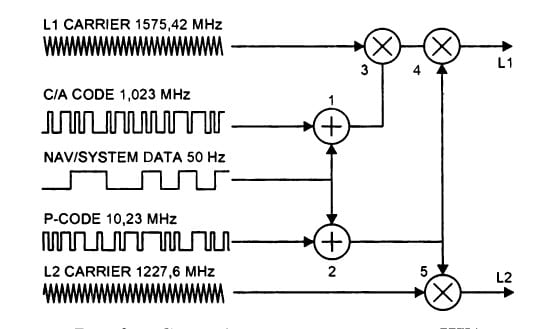
\includegraphics[width=0.7\linewidth]{fig/fig-1.jpg}    
\caption{Схема формирования сигналов GPS \cite{4}.}
\label{fig-1}      
\end{figure}
 
GPS использует специальную непрерывную шкалу времени без поправок на високосные секунды GPST (от англ. GPS Time), которая берёт своё начало 6 января 1980 года в 0:00 UTC (от англ. Coordinated Universal Time).
Эпоха GPST определяется через номер недели GPS и номер секунды в неделе. 
Иногда (для удобства) ещё используется номер дня в неделе, отсчёт которых берёт своё начало в воскресенье.
Например, 1 января 2020 года 0:00 UTC соответствует 2086 недель GPS и 259200 секунд.

Проект GPS постоянно модернизируется.
В настоящее время существует и функционирует несколько типов спутников GPS.
Их список представлен в табл. \hyperref[tab-1]{1}.
Созвездие GPS включает в себя 32 действующих спутника, 31 из которых используется по целевому назначению и 1 выведен на техобслуживание. 
Также постепенно интегрируется новые коды для модуляции сигналов: L2C-код для сигнала L2, L5C-код для нового общедоступного сигнала L5 (1176,45 МГц), M-код для замены старого Y-кода.

\begin{table}[h]
\centering
\begin{tabular}{|c|c|c|c|}
\hline
Блок  & Период запусков     & Работают сейчас & На техобслуживании \\ \hline
I     & 1978—1985           & 0               & 0                  \\ \hline
II    & 1989—1990           & 0               & 0                  \\ \hline
IIA   & 1990—1997           & 0               & 0                  \\ \hline
IIR   & 1997—2004           & 10              & 0                  \\ \hline
IIR-M & 2005—2009           & 7               & 1                  \\ \hline
IIF   & 2010—2016           & 12              & 0                  \\ \hline
III   & 2018—2023           & 2               & 0                  \\ \hline
\end{tabular}
\caption{Список запусков спутников GPS \cite{5}.}
\label{tab-1}
\end{table}